\documentclass[12pt,fleqn]{article}
\setlength{\parindent}{0pt}
\usepackage{graphicx}
\usepackage{cancel}
\usepackage{listings}
\usepackage[latin5]{inputenc}
\setlength{\parskip}{8pt}
\setlength{\parsep}{0pt}
\setlength{\headsep}{0pt}
\setlength{\topskip}{0pt}
\setlength{\topmargin}{0pt}
\setlength{\topsep}{0pt}
\setlength{\partopsep}{0pt}
\setlength{\mathindent}{0cm}

\begin{document}
Dalga Denklemini Turetmek 

PDE'lerin ortaya cikabilecegi durumlardan biri, ayriksal parcaciklardan
olusan bir sistemin limite gittigi andir. Bu tur sartlarda ODE'lerden
olusan bir sistem limite giderken bir PDE ortaya cikartabiliyor. Sureklilik
Mekaniginden (Continuum Mechanics) bir ornek verecegiz yani.

Sistem ayriksal baslayacak, sureklilik limitine gidecek. Mesela sivilar
mekaniginde (fluid mechanics) Euler denklemi, Navier-Stokes denklemleri
sivi sisteminin (su gibi mesela) sureklilik limitidirler. Bu denklemler
sivi icindeki ufak parcaciklari tarif etmezler, sistemin butunune
bakarlar. 

Hepimiz Newton Kanunu biliyoruz (ki bu kanun bu derste ihtiyacimiz olan
yegane fizik bilgisi)

\[ m \frac{d^2x}{dt^2} = F(x) \]

Formul ne diyor? Kutle carpi ivme esittir kuvvet. Gayet basit.

Diyelim ki elimizde $N$ tane tane parcacik var, $i=1,..,N$, ve bu
parcaciklar birbirleriyle etkilesim halindeler, aralarinda bir tur cekim
var belki, ya da baska bir kuvvet. O zaman her parcacik icin ayri ayri
hareket kanunu isleyecek. Ve $i$'inci parcacik uzerinde bir kuvvet var, ve
bu kuvvet sistemdeki tum diger degiskenlerle bir sekilde bagimli. $x$ tabii
ki pozisyon degiskeni. O zaman

\[ m_i \frac{d^2x_i}{dt^2} = F_i(\vec{x}) \]

Dikkat edersek, $F$ fonksiyonuna giren parametre tum parcaciklar, yani o
parcacigin hissettigi kuvvet bir sekilde tum diger parcaciklarla alakali. 

Baslangic Sarti

$i$'inci parcacigin baslangic konumu

\[ x_i(0) = \hat{x}_i \]

Tipik olarak baslangic hizi da verilir

\[ \frac{dx_i}{dt}(0) = \hat{v}_i \]

Ustteki bir baslangic deger problemi (initial value problem). Biz bu derste
PDE bazinda sinir degerli problemlerle ugrasacagiz. 

Bu tur baslangic deger problemleri iyi huyludur, cunku, mesela bu ornekte
2. derece bir diferansiyel denklem var elimizde, ve bagimli degisken $x$
var, ve bize verilen kosulu anlamak icin alttaki resme bakalim


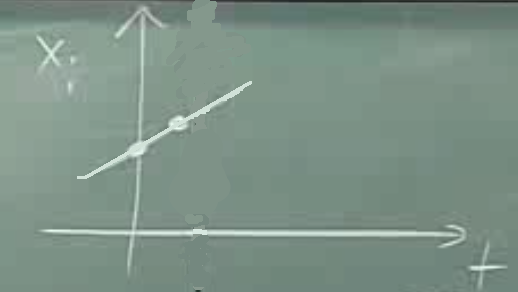
\includegraphics[height=3cm]{1_06.png}

Bize verilenler, $t=0$ aninda $x_i$ noktasinin oldugu yere ek olarak
(soldaki nokta), bir de o noktadaki egim bilgisi. Bu tur bilgi verilince,
parcacigin hangi yone gitmeye meyilli olacagini da gormus oluyoruz. Sanki
bir top ateslenmis, ve topun ates ettigi anda nerede olduguna ek olarak
topun namlusunun gosterdigi yer de bize soyleniyor.

Bu iyi huylu bir problem. Sinir degerli denklemler cok daha karmasik
olabiliyor. Bu arada ``sinir kosullu'' kelimesindeki ``sinir'' cogunlukla
bir fiziksel seye tekabul eder, mesela bir ip vardir, ve ipin ``sonunda''
yani sinirlarinda degerin ne olmasi gerektigi sabitlenir. 

Devam edelim. Kurmak istedigimiz model bir tur ``gitar teli'' modeli. 

$y_i$ = $i$'inci parcacigin yuksekligi olsun. 

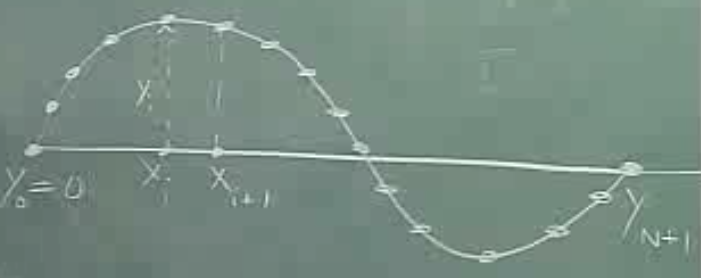
\includegraphics[height=4cm]{1_07.png}

Tel uzerinde bir suru parcacik var, tel iki ucundan sabitlenmis durumda. Bu
problemde yatay hareketle ilgilenmiyoruz, sadece yukari / asagi hareketle
ilgileniyoruz. Bir tanim daha:

\[ \Delta x = x_{i+1} - x_i  \]

Basitlestirme amaciyla bu tanimi yaptik. Tum parcaciklarin arasindaki
mesafeyi sabit, ve ayni olarak aldik. Benzer sekilde

\[ m_i \equiv m \]

Yani tum parcaciklar ayni kutleye sahip. 

Simdi Newton Kanununu parcaciklara uygulayalim [1]. 

\[ m \frac{d^2Y_i}{dt^2} = 
\tau \bigg( \frac{Y_{i+1}- Y_i}{\Delta x} \bigg) -
\tau \bigg( \frac{Y_{i}- Y_{i-1}}{\Delta x} \bigg) 
\]

Bununla ne demis olduk? $i$'inci parcacigin hissettigi cekimin, o
parcacigin saginda ve solunda bagli oldugu diger parcacikla baginin ipteki
egimi ile orantili oldugunu soylemis olduk.

$\tau$ her tel icin farkli olacak bir gerginlik sabiti, ama belli bir
telde, her parcacik icin ayni. 

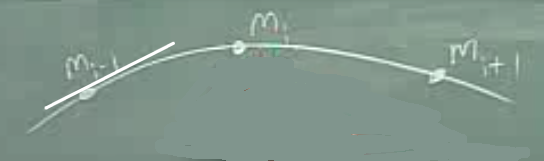
\includegraphics[height=3cm]{1_08.png}

Ustteki formul aslinda yerel turevin ``ucuz'' bir yaklasiksallamasi. 

Gerginlikle kurulan alaka akla yatkin olmali, dusunursek ipte parcacik ne
kadar yuksekte olursa uzerinde o kadar guc hissederdi, yanindaki
parcaciklar(lar) tarafindan asagi cekilirdi, ne kadar altta ise o kadar az
guc hissederdi. Tabii ``diger parcaciklara gore'' yukarida ya da asagida
olmanin olcusu de iki parcacik arasindaki ipin egimi. 

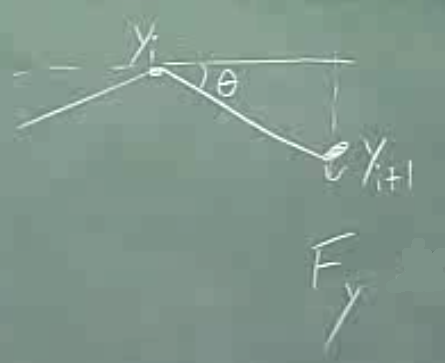
\includegraphics[height=4cm]{1_09.png}

Diger bir acidan yaklasirsak

\[ F_y \equiv \tau sin\theta \]

da diyebilirdik. Sadece sin kullandik cunku daha once belirttigimiz gibi,
sadece dikey hareketlere bakiyoruz, yatay hareketlerle ilgilenmiyoruz (o
yuzden cos yok).

Bir yaklasiksallama yapabiliriz simdi, eger $\theta << 1$ ise, yani aci 1
sayisindan cok kucuk ise, $sin\theta \approx tan\theta$ sayilabilir, bu
sonuc Taylor Serileri ile alakali ve $tan$ fonksiyonu, $sin / cos$ oldugu
icin ve sifira yakin degerlerde bolen $\theta$'nin sifira yakinligindan cos
uzerinden hep 1'e yakin olacagi icin, $tan$ bir nevi $sin$
sayilabilir. Peki bu problemde $tan\theta$ nasil hesaplanir?

\[  \tan\theta = \frac{\Delta y}{\Delta x} \]

\[ = \frac{Y_{1+1}-Y_i}{\Delta x} \]

Yani yine ayni yere gelmis olduk. 

Bu model bir ``en yakin komsu'' modelidir, her parcacik yakinindaki
parcaciktan etkileniyor. 

Ana formulu su sekilde tekrar organize ederek yazalim

\[ \frac{d^2Y_i}{dt^2} = 
\tau \frac{\Delta x}{m} \bigg[
\frac{Y_{i+1} - 2Y_i + Y_{i-1}}{\Delta x^2}
\bigg]
\]

Koseli parantez icindeki ifade Calculus'ta 2. turevin ayriksal formdaki
yaklasiksallamasi degil mi?

Ayriksal modelimiz boyle. Simdi sureklilik limitine gecmek istiyorsak,
mesela sonsuz sayida parcacik oldugu bir duruma gecmek isteyebiliriz,
$\lim_{N \to \infty}$, elimizde sonlu / belli miktarda bir tel var, bu durumda 
sonsuz sayida parcacik demek bu parcaciklarin arasindaki mesafenin sifira 
gitmesi demektir, o zaman $\lim_{\Delta x \to \infty}$. 

Formul icin bunun anlami nedir? $\Delta x$ ve $m$ arasindaki oran sonlu
(finite) bir sayiya yaklasacak demektir, ki bu sayiya yogunluk
diyebiliriz. Oran niye sifira gitmiyor? Sureklilik sistemlerin kullanilan
bir numara bu,

\[ \rho = \lim_{\Delta x \to 0} \frac{m}{\Delta x} \]

$\Delta x$'in asagi indigini dusunuyoruz, ama olabilecek cok ufak bir hacim
hayal ederek mesela molekul boyutundan daha fazla asagi inmeyecegini
soyluyoruz, $m$ ayni sekilde kuculuyor, ve oran bize bir yogunluk hesabi
veriyor.

Taylor Serileri hakkinda hizli bir ders

\[ Y_{i+1}=Y(x_i + \Delta x) \]

Eger $\Delta x$ cok kucuk ise

\[ = 
\underbrace{Y(x_i)}_{Y_i} + \Delta x \frac{dY}{dx}|_{x_i} + 
\frac{\Delta x^2}{2}\frac{dY^2}{dx^2}|_{x_i} + 
O(\Delta x^3)
\]

Daha kisa bir sekilde yazalim

\[ Y_{i+1} = Y_i + \Delta x Y_i' + \frac{\Delta x^2}{2}Y_i'' + ... 
\]

Ayni seyi $Y_{i-1}$ icin yapabiliriz

\[ Y_{i-1} = Y_i - \Delta x Y_i' + \frac{\Delta x^2}{2}Y_i'' + ... 
\]

Not: Esitligin sagindaki eksi, arti isaretlerinin nereden geldigini merak
ediyorsak, Hesapsal Bilim 1 Ders 2 notlarinda $u(x-h)$ acilimina
bakabiliriz.

Son iki formulu toplarsak

\[ Y_{i+1} + Y_{i-1} = 2Y_i + \Delta x^2 Y_i''  + O(\Delta x^4)\]

O zaman 2. turevin $x_i$'daki yaklasiksallamasi 

\[ Y_i'' = \frac{Y_{i+1} - 2Y_i + Y_{i-1}}{\Delta x^2} + O(\Delta x^2) \]

O zaman ana formulde

\[ \frac{d^2Y_i}{dt^2} = 
\tau \frac{\Delta x}{m} \bigg[\underbrace{
\frac{Y_{i+1} - 2Y_i + Y_{i-1}}{\Delta x^2}
}_{\to \frac{\partial ^2y}{\partial x^2}}
\bigg]
\]

Yani $\Delta x \to 0$ iken koseli parantez ici $\partial ^2y/\partial
x^2$'e gider. Niye kismi tureve gider? Cunku ayriksal degisimi sadece $x$
uzerinde yaptik, fakat $Y$ icinde ayni zamanda $t$ de var. Notasyon olarak
ODE dili kullanmamiz kafa karistirmasin, goruntu basit olsun diye bunu
yaptik. Ama degisimin $x$ te olmasi sebebiyle turev kismi turev oldu. 

O zaman bu sistemin sureklilik limiti, $\Delta x \to 0$ iken

\[ 
\frac{\partial ^2Y}{\partial x^2} = 
\frac{\tau}{\rho}\frac{\partial ^2y}{\partial x^2}
 \]

olacaktir. Bu denklem fizikte iyi bilinen dalga denklemidir. Insanlar
cogunlukla 

\[ c^2 = \frac{\tau}{\rho} \]

seklinde yazarlar ve $c$ boylece ``dalga hizi'' olarak kullanilabilir. 

Eger teli bir noktasinda titrettigimiz dusunursek, ve telin sonlu degil
sonsuz oldugunu dusunelim, o zaman ``hareket eden dalgalar (traveling
waves)'' fenomenini goruruz. Alttaki resimde $t=0$ aninda bir tepe noktasi
var (tele vurduk), ve ikinci resimde iki tane tepe noktasi saga ve sola
esit sekilde hareket ediyorlar. 

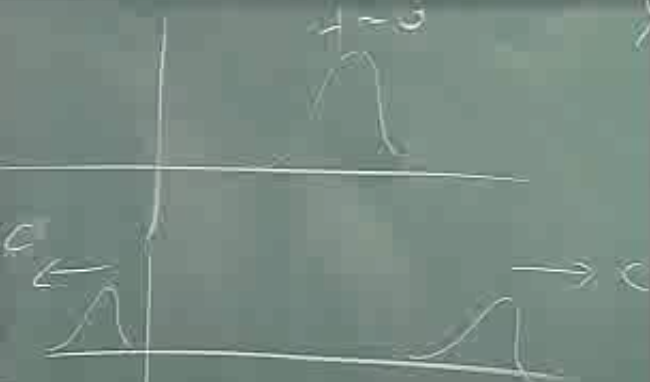
\includegraphics[height=3cm]{1_10.png}

PDE'ler ayriksal sistemlerin, ODE'lerin, sureklilik limitinde dogal olarak
ortaya cikarlar. Bu tur yaklasiksallamalari ben arastirmalarimda surekli
kullaniyorum [hoca uygulamali matematikci], akiskanlik mekaniginde mesela,
bir sivinin, molekulun kisimlarini aliyoruz, ve kisimlar birbirleri ile
etkilesimde oluyorlar. Ya da mesela yogunluk degiskenini, kutleyi bir
surekli fonksiyon haline getiririz, ve parcacik hizi yerine sivinin
tamaminin hizina bakariz. Yani bu cok kullanilan bir teknik. Cogunlukla
ayriksal bir ag yapisi icin analitik bir denklem bulmak cok zordur, o
sebeple sureklilik yaklasiksallamasi kullanilir zaten. Belki ustteki
problem icin alternatif cok kotu olmayabilirdi, mesela burada ODE'leri
matris formunda yazarak ta cozume gidebilirdik, bu cok zor olmazdi, fakat
cogu zaman bunu yapmak hakikaten zor olabiliyor.

Niye sistemi analitik olarak gormek istiyoruz? Cunku o zaman formulasyonu
istedigimiz gibi manipule ederek, analitik sekilde istedigimiz yoldan
ilerleyebiliyoruz.

* * *

Bir PDE kategorisinden bahsedelim, bu tur PDE'ler en cok kullandigim
PDE'lerden, lineer 1. derece denklemler. Ve bu arada ``karakteristikler''
kavramindan bahsedecegiz. 

1. Derece, Lineer PDE, 2 Bagimsiz Degisken

\[ u = u(x,y) \]

PDE

\[ a(x,y)u_x + b(x,y)u_y + c(x,y)u = f(x,y) \]

Operator olarak 

\[ \mathcal{L}u = f \]

\[ \mathcal{L} = a \frac{\partial }{\partial x} +
b \frac{\partial }{\partial y} +
c \frac{\partial }{\partial z} 
\]

Karakteristik kavramindan birazdan istifade edecegiz, ama simdi bu tur
denklemleri kaba kuvvet kullanarak, ``degisken degistirme (change of
variables)'' yontemi ile nasil cozulebilecegini gosterelim. 

Tanim

Cauchy Problemi: $u(\vec{x})$ tanimi gerektirir. Bu tur problemler
1. derece, 2 degisken, vs. gibi tanimlarla sinirli degil aslinda, cok daha
genel bir tanim onlar, bu tur problemlerde bir ``Caucy Verisi (Cauchy
Data)''nden bahsedilir.

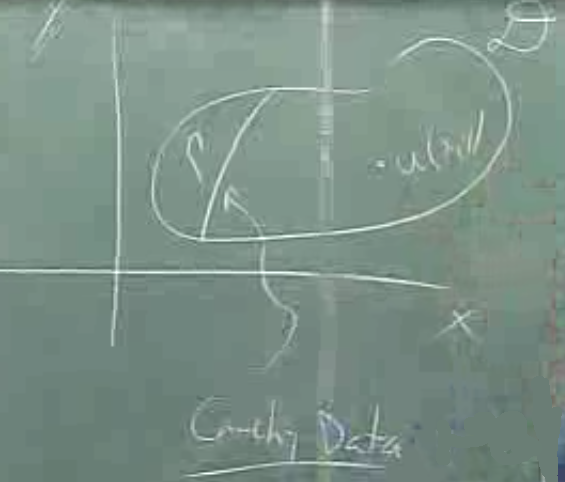
\includegraphics[height=4cm]{1_11.png}

Ustteki resimde bu veri $D$ alani (domain) icindeki $\Gamma$ ile isaretli
cizgidir, ki $u$'nun bu cizgi uzerindeki degeri diyelim ki

\[ u|_{\Gamma} = \alpha(x,y) \]

ki $\alpha(x,y)$ herhangi bir sonuc. 

Mesela $\Gamma$ cizgisi $x=sin(y)$ ile tanimli egri, ve $u$ onun uzerinde
$u=y^2$ olmali.

Bu tur bir kosula Cauch Verisi ismi veriliyor, bizim ornegimizde bu bir tur
sinir kosulunu andiriyor. 

Bir kordinat sistemi nedir? 

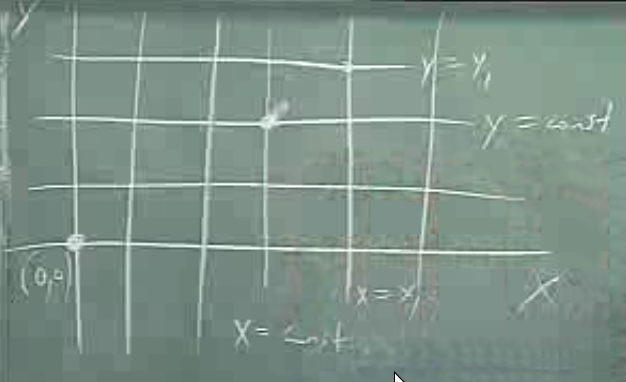
\includegraphics[height=4cm]{1_12.png}

Diyelim ki oyle bir fonksiyon kumesi var ki, onlar uzerinden PDE'lerimizi
degisik bir kordinat sisteminde temsil etmemiz mumkun olacak. 

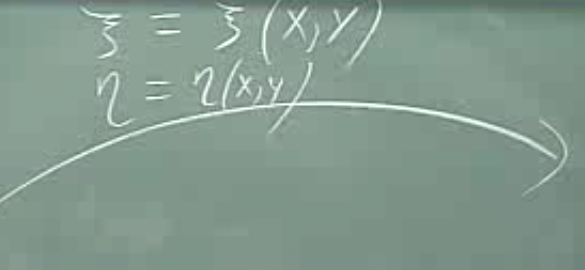
\includegraphics[height=2cm]{1_13.png}

$\xi$ ve $\eta$'yi kesit egrileri (level curves) uzerinden incelemek
mumkundur. Bu fonksiyonlari belli sabitlere esitleyip, durumlarina
bakabiliriz, sonra sabitleri degistiririz, bir daha bakariz, vs. 

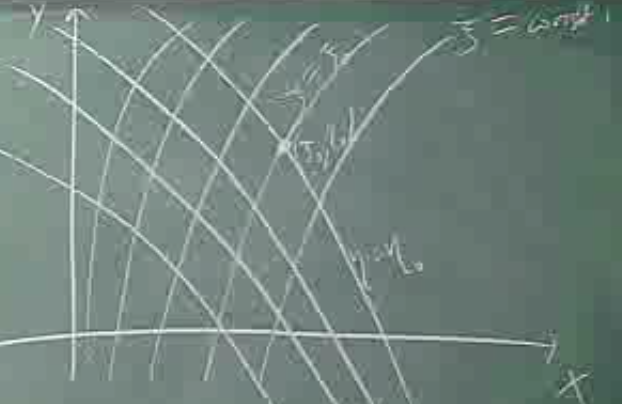
\includegraphics[height=6cm]{1_14.png}

Ustteki resimde mesela, saga yatik tum egriler, her biri degisik bir sabite
(Ingilizce const diye yazilmis) esit olacak sekildeki $\xi$ egrileri
olabilir. Sola yatik $\eta$ cizgileri de olabilir. Ortadaki nokta iki
onceki resimdeki bir noktanin bu yeni kordinata eslenmis bir nokta mesela.

Gerekliliklerimiz

Esleme, transformasyon bire bir (one-to-one) olmali. Ilk kordinat
sistemindeki her nokta, diger kordinat sistemindeki tek bir noktaya
esleniyor olmali. 

Jacobian'i yokolmayan (non-vanishing) olmali. 

\[ 
\left(\begin{array}{rr}
\xi & \eta \\
x & y
\end{array}\right) = 
\left|\begin{array}{rr}
\xi_x & \xi_y \\
\eta_x & \eta_y
\end{array}\right| =
\xi_x \eta_y - \xi_y \eta_x \ne 0
 \]

Ustteki ifade Calculus'un Dolayli Fonksiyon Teorisi (Implicit Function
Theorem of Calculus) ile alakali. Bu teorinin yerel baglamda niye birebir
esleme yarattigini merak ediyorsaniz Calculus kaynaklarina
danisabilirsiniz. 

Amac: Sunu 

\[ au_x + bu_y + cu = f \]

transform et ve suna cevir

\[ W_\xi + h(\xi, \eta)W = R(\xi,\eta)\]


\[ W(\xi,\eta) \equiv u \bigg( x(\xi,\eta),y(\xi,\eta) \bigg) \]

Birebir transformasyon istemistik, o zaman esleme geriye cevirilebilir
(invertible) de olmali, yani istersek $x,y$ degiskenlerini $\xi,\eta$
cercevesinde temsil edebiliyor olmamiz lazim. 

Dikkat: $W_\eta$ yoktur, bu sayede iki ustteki formul 1. derece ODE haline
gelir, entegre edici faktor kullanip entegre edip Cauchy Verisini
uygulayarak bu problemi cozebilirsiniz. Analitik olarak biraz karmasikliga
sebep verebilir, ama bu en azindan mumkun bir stratejidir. 

Simdi sira transformasyonu bulmaya geldi. $x,y$ degiskenlerini $\xi,\eta$
cercevesinde temsil edelim. Zincirleme Kanununu kullanalim. 

\[ \frac{\partial }{\partial x}u \equiv
\frac{\partial }{\partial x}W(\xi(x,y),\eta(x,y)) =
W_\xi\eta_x + W_\eta\eta_x 
 \]

\[ \frac{\partial }{\partial y}u =
W_\xi\eta_y + W_\eta\eta_y
 \]

Bunu orijinal denkleme sokalim

\[ 
a(\xi,\eta) \bigg[W_\xi \eta_x + W_\eta\eta_x \bigg] +
b(\xi,\eta) \bigg[W_\xi \eta_y + W_\eta\eta_y  \bigg] + 
c(\xi,\eta)W = f(\xi,\eta)
 \]

Tekrar duzenleyelim

\[ = 
\bigg[ a\xi_x + b\xi_y \bigg] W_\xi + 
\bigg[ a\eta_x + b\eta_y \bigg] W_\eta +
cW = f
 \]

Soyle sec

1.

\[ a \eta_x + b \eta_y = 0 \]

\[ \Rightarrow \frac{\eta_x}{\eta_y} = -\frac{b(x,y)}{a(x,y)}\]

2. 

\[ \xi = x \]

Boylece 

\[ h = \frac{c}{a} \]

\[ R = \frac{f}{a} \]

elde edilir. 

Unutmayalim Jacobian sartini tatmin etmemiz lazim. 

Farz edelim 

\[ \eta_y \ne 0 \]

Bu ise yarar

\[ J = \xi_x\eta_y - \cancelto{0}{\xi_y}\eta_y \]

\[ J = \eta_y \ne 0 \]

Bir dahaki derste $\eta$'yi nasil hesaplayacagimizi gorecegiz. 

---

[1] Diger bir acidan bakarsak, mesela matematikci David Mumford
turetirken ($i$ yerine $k$ kullanmis)

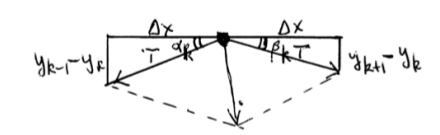
\includegraphics[height=3cm]{1_15.png}

\[ 
\tau \bigg( \frac{Y_{i+1}- Y_i}{\Delta x} \bigg) +
\tau \bigg( \frac{Y_{i-1}- Y_{i}}{\Delta x} \bigg) 
\]

kullanmis. Yani bir parcacigin uzerindeki kuvvet sagindaki ve solundaki
kuvvetlerin ``toplami'' olarak goruluyor, bu formul de ayni kapiya cikiyor.


PDE - Isi Denklemini Turetmek - Ders 2

Denklem soyle idi

\[ a(x,y)u_x + b(x,y)u_y + c(x,y)u = f(x,y) \]

Bu denklem homojen degil, cunku denklemin sol tarafi $f \ne 0$, homojenlik
icin nihai test tabii ki $u=0$ koyunca $0=0$ cikip cikmayacagi.

Cozum icin kullandigimiz fikir neydi? Kordinat sistemini transform etmek,
ki 

$\bigg(x,y\bigg) \to \bigg(\xi(x,y), \eta(x,y)\bigg)$

olsun. Bu degisimi yaparken oyle bir degisim ariyoruz ki boylece transform
edilmis PDE'miz cozulmesi kolay bir hale gelsin. 

Amac

Denklemi sadece tek bir bagimsiz degiskene gore turevi icerecek sekilde
yazmak 

\[ w_\xi + h(\xi,\eta)w  = R(\xi,\eta) \]

\[ w \equiv u \bigg( x(\xi,\eta),y(\xi,\eta) \bigg)  \]

\[ 
J = 
\left|\begin{array}{rr}
\xi_x & \xi_y \\
\eta_x & \eta_y
\end{array}\right| =
\xi_x \eta_y - \xi_y \eta_x \ne 0
 \]

Turev Transformasyonu

\[ \frac{\partial }{\partial x} = 
\frac{\partial \xi}{\partial x}  \partial_\xi + 
\frac{\partial \eta}{\partial x}\partial_\eta
\]

\[ \frac{\partial }{\partial y} = 
\frac{\partial \xi}{\partial y}  \partial_\xi + 
\frac{\partial \eta}{\partial y}\partial_\eta
\]

Bunu yapinca PDE su hale gelecek

\[ a \bigg[ a\xi_x + b\xi_y \bigg]w_\xi + 
a \bigg[ a\eta_x + b\eta_y \bigg]w_\eta + 
cw = f
 \]

Simdi $\eta$ kordinatini oyle bir sekilde secmek istiyoruz ki ustteki sag
koseli parantez icindeki terimler yokolsun. Boylece PDE'yi $\xi$ bir ODE'ye
indirgemis oluruz. Bunu elde edince entegrasyon kolaylca yapilabilir. 

\[ a \eta_x + b\eta_y = 0 \]

\[=> \frac{\eta_x}{\eta_y} = - \frac{b(x,y)}{a(x,y)} \]


Yani ikinci kordinat sistemi her ne ise, onun ortaya cikardigi kismi
turevlerinin birbirine orani katsayi fonksiyonlarinin oraninin negativine
esit.  

[burada kesildi]



\end{document}
